\documentclass{beamer}
\usetheme{Madrid}
\usecolortheme{beaver}
\usepackage{textpos}

\title{TRIUMF nEXO SiPM Studies}
\author[]{
\includegraphics[height=2.0cm,width=2.2cm]{./EXO.png}~\\  ~\\Fabrice Reti\`{e}re\\Carl Rethmeier\\Lloyd James\\Paul Lopes Gomes\vspace{-0.5cm}}
\institute[]{
\includegraphics[height=0.8cm,width=2.5cm]{./TRIUMF.png}}
\date{\today}

\setbeamertemplate{footline}
{
  \leavevmode%
  \hbox{%
  \begin{beamercolorbox}[wd=.333333\paperwidth,ht=2.25ex,dp=1ex,right]{author in foot/foot}%
    \usebeamerfont{author in foot/foot}\insertshortauthor%~~\beamer@ifempty{\insertshortinstitute}{}{(\insertshortinstitute)}
  \end{beamercolorbox}%
  \begin{beamercolorbox}[wd=.333333\paperwidth,ht=2.25ex,dp=1ex,center]{title in foot/foot}%
    \usebeamerfont{title in foot/foot}\insertshorttitle
  \end{beamercolorbox}%
  \begin{beamercolorbox}[wd=.333333\paperwidth,ht=2.25ex,dp=1ex,right]{date in foot/head}%
    \usebeamerfont{date in foot/head}\insertshortdate{}\hspace*{2em}
    \insertframenumber{} / \inserttotalframenumber\hspace*{2ex} 
  \end{beamercolorbox}}%
  \vskip0pt%
}
\makeatother


\begin{document}

\begin{frame}
\maketitle
\end{frame}

\addtobeamertemplate{frametitle}{}{%
\begin{textblock*}{100mm}(.85\textwidth,-1cm)
\vspace{0.5mm}
\hspace{-2.5cm}

\includegraphics[height=0.8cm,width=2.5cm]{./TRIUMF.png}
\hspace{0.5cm}

\includegraphics[height=0.9cm,width=0.9cm]{./EXO.png}
\end{textblock*}}

\begin{frame}{Pulse Amplitude vs Time - VUV3}
\begin{figure}
\centering
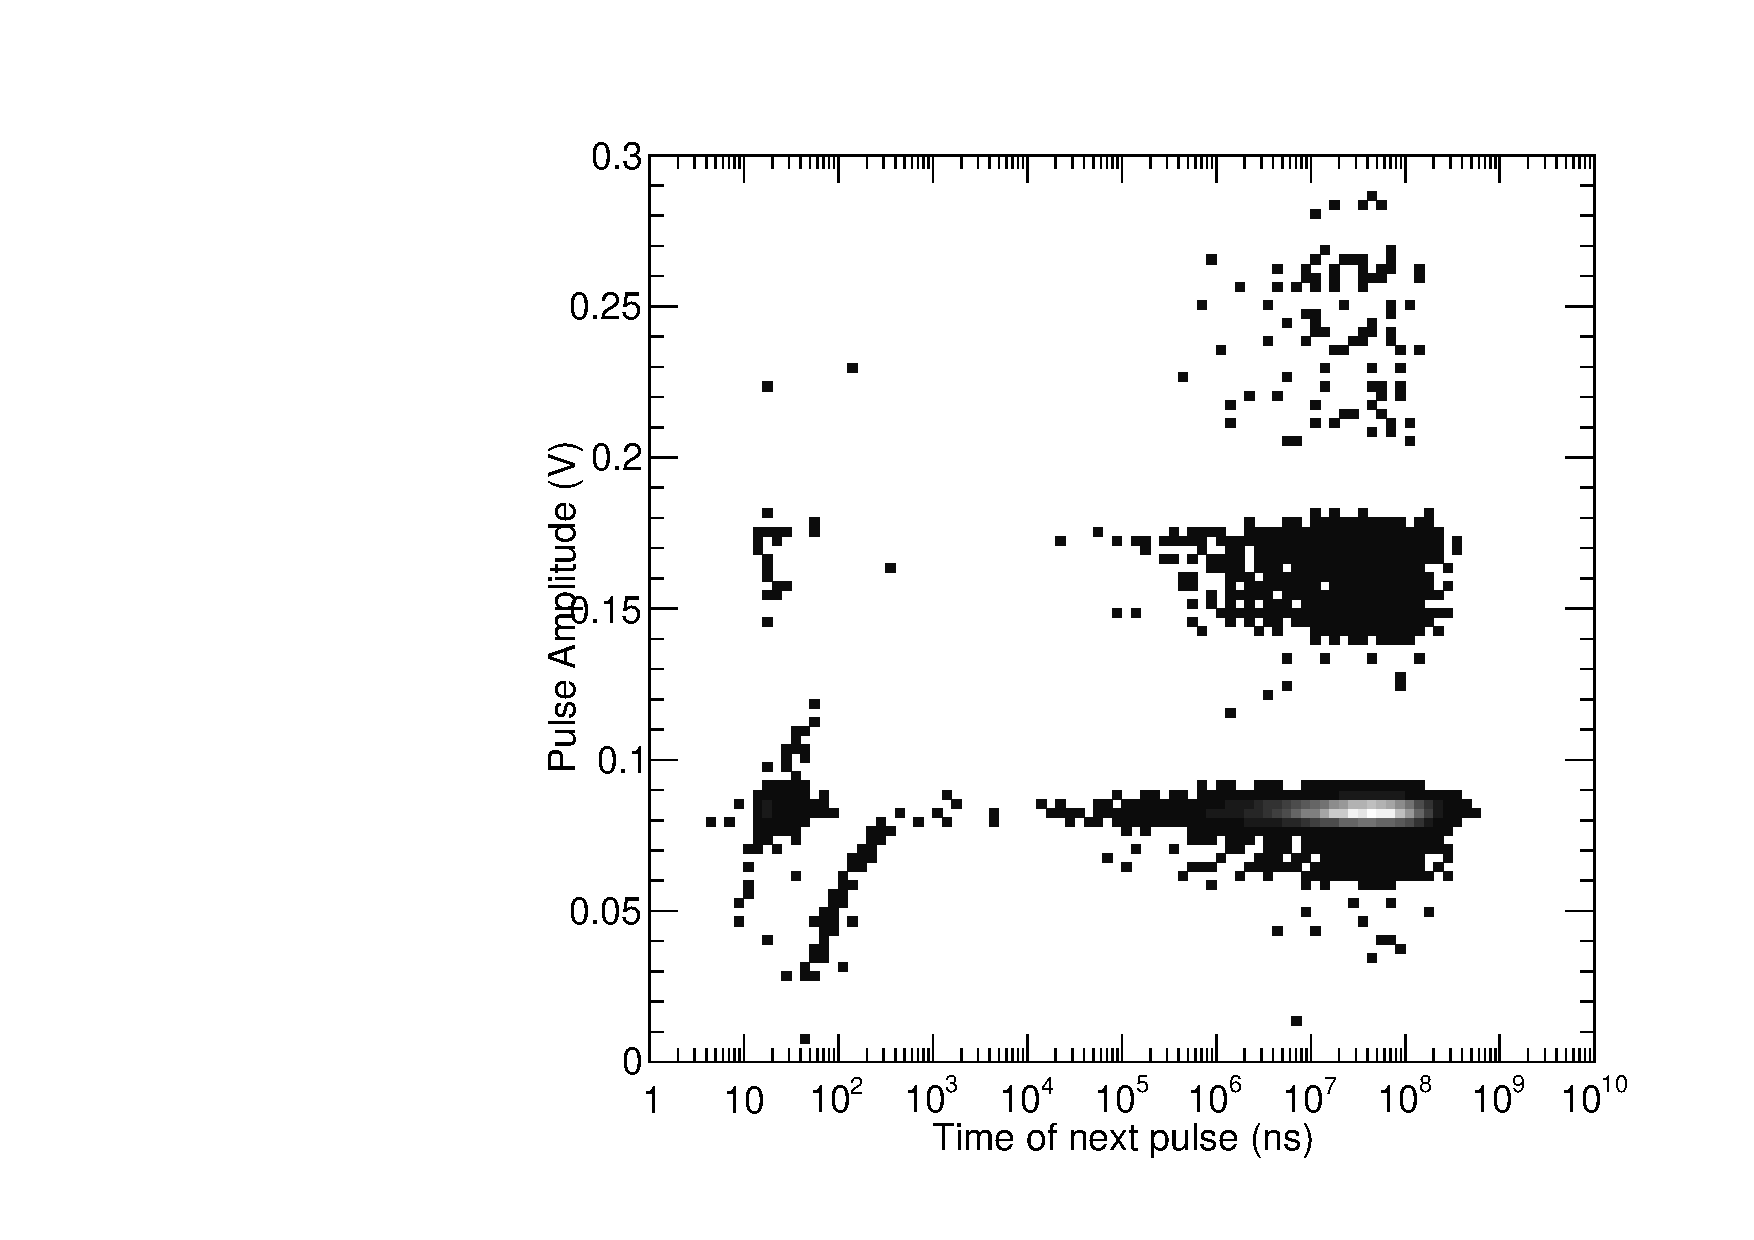
\includegraphics[height=0.5\textwidth]{AmpVUV3.pdf}%
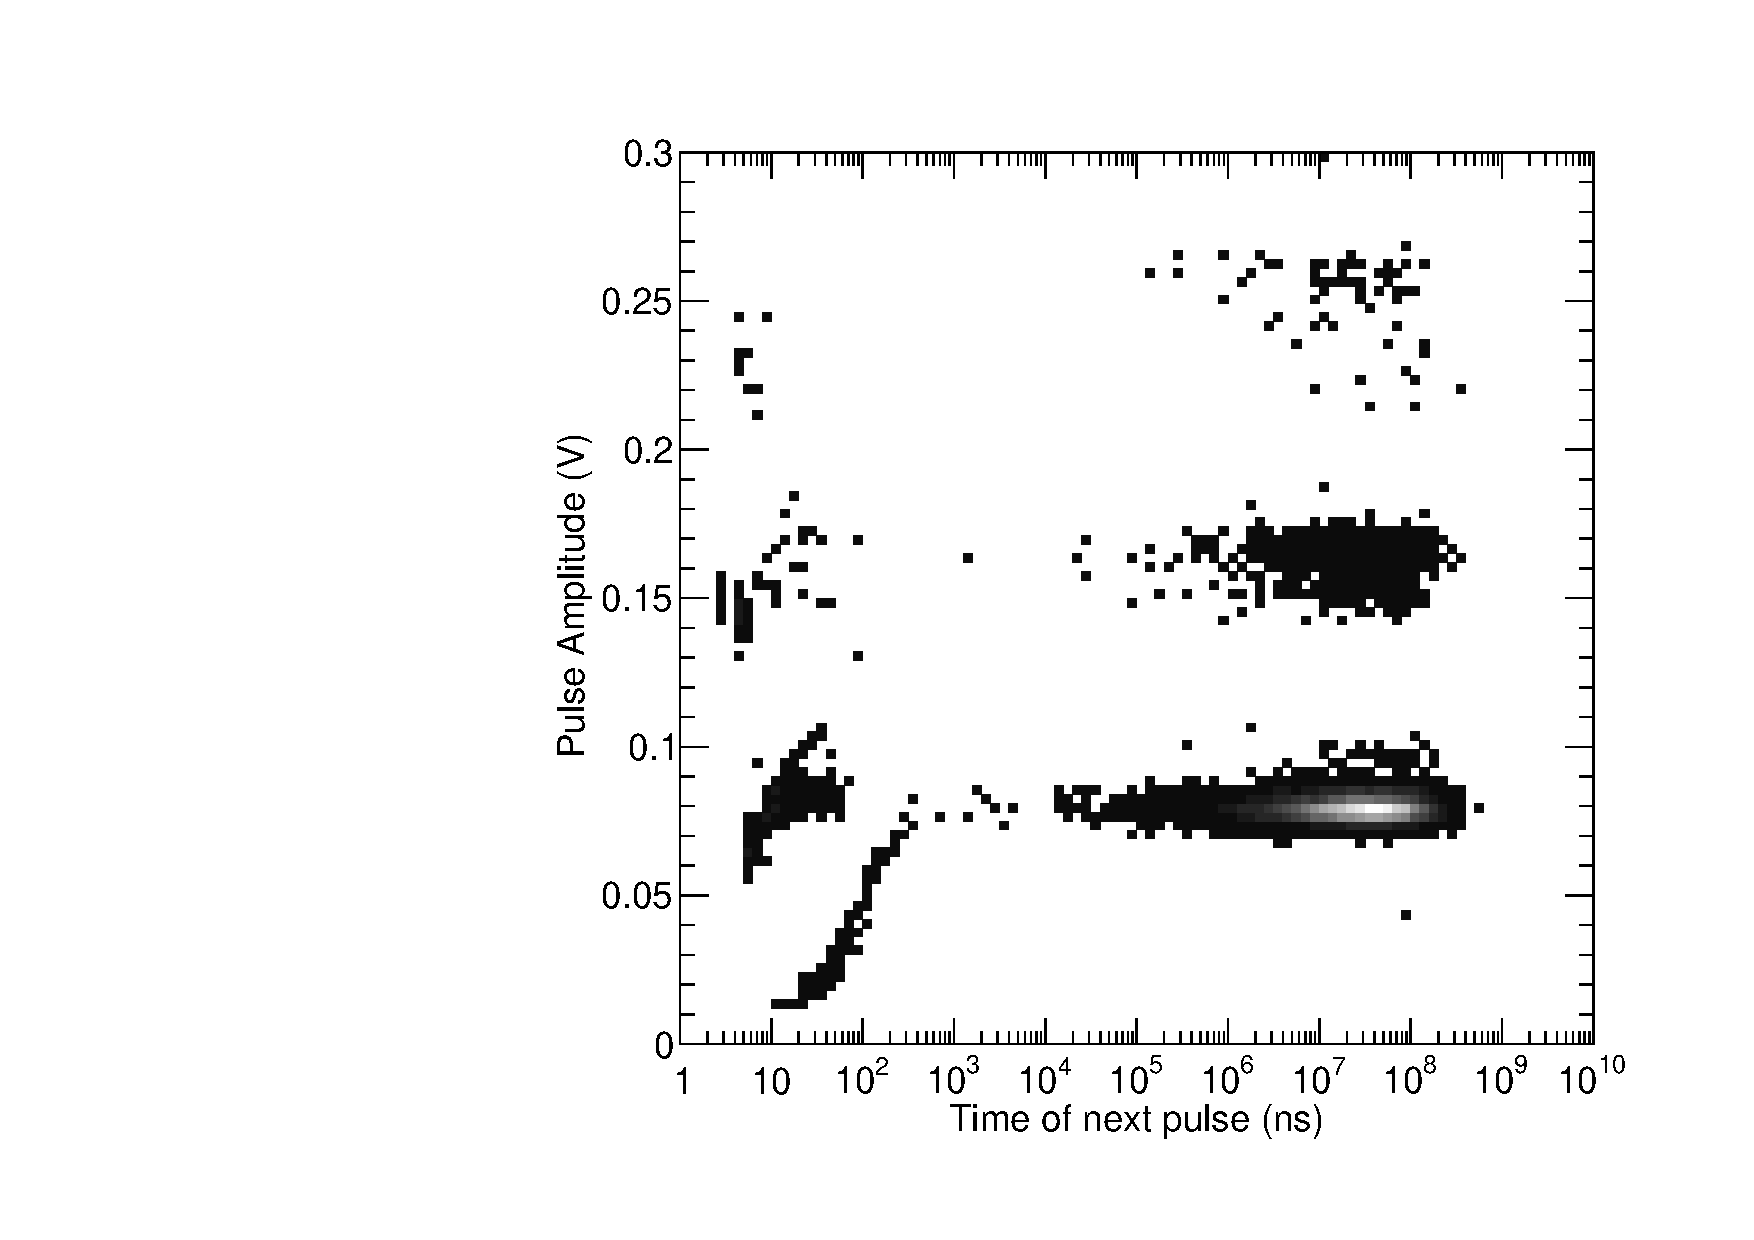
\includegraphics[height=0.5\textwidth]{AmpVUV3_new.pdf}
\caption{Amplitude of pulses against the time between the pulse and the previous pulse, before and after improvements to the pulse finder. No fitting involved.}
\end{figure}
\end{frame}

\begin{frame}{Band Spreading - VUV3}
\begin{figure}
\centering
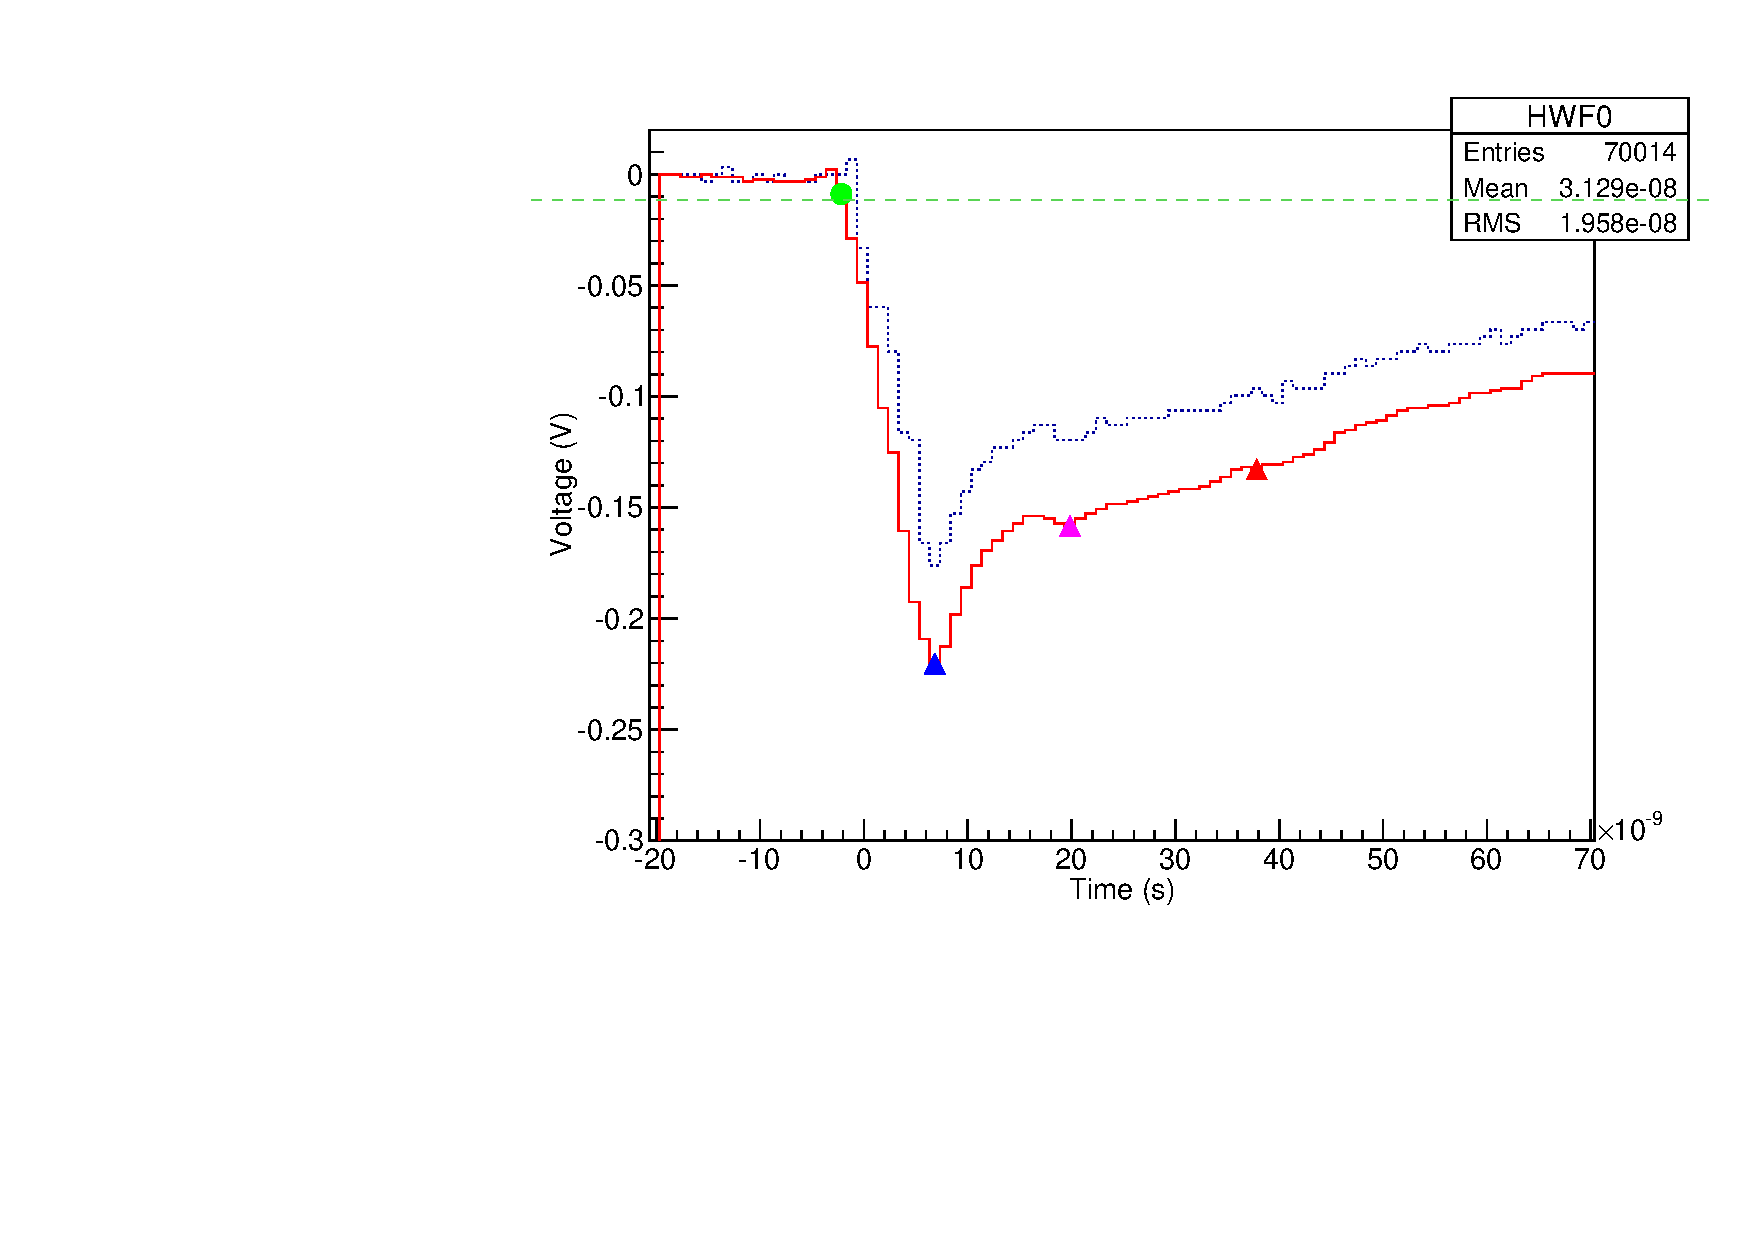
\includegraphics[height=0.38\textwidth]{peak_low.pdf}%
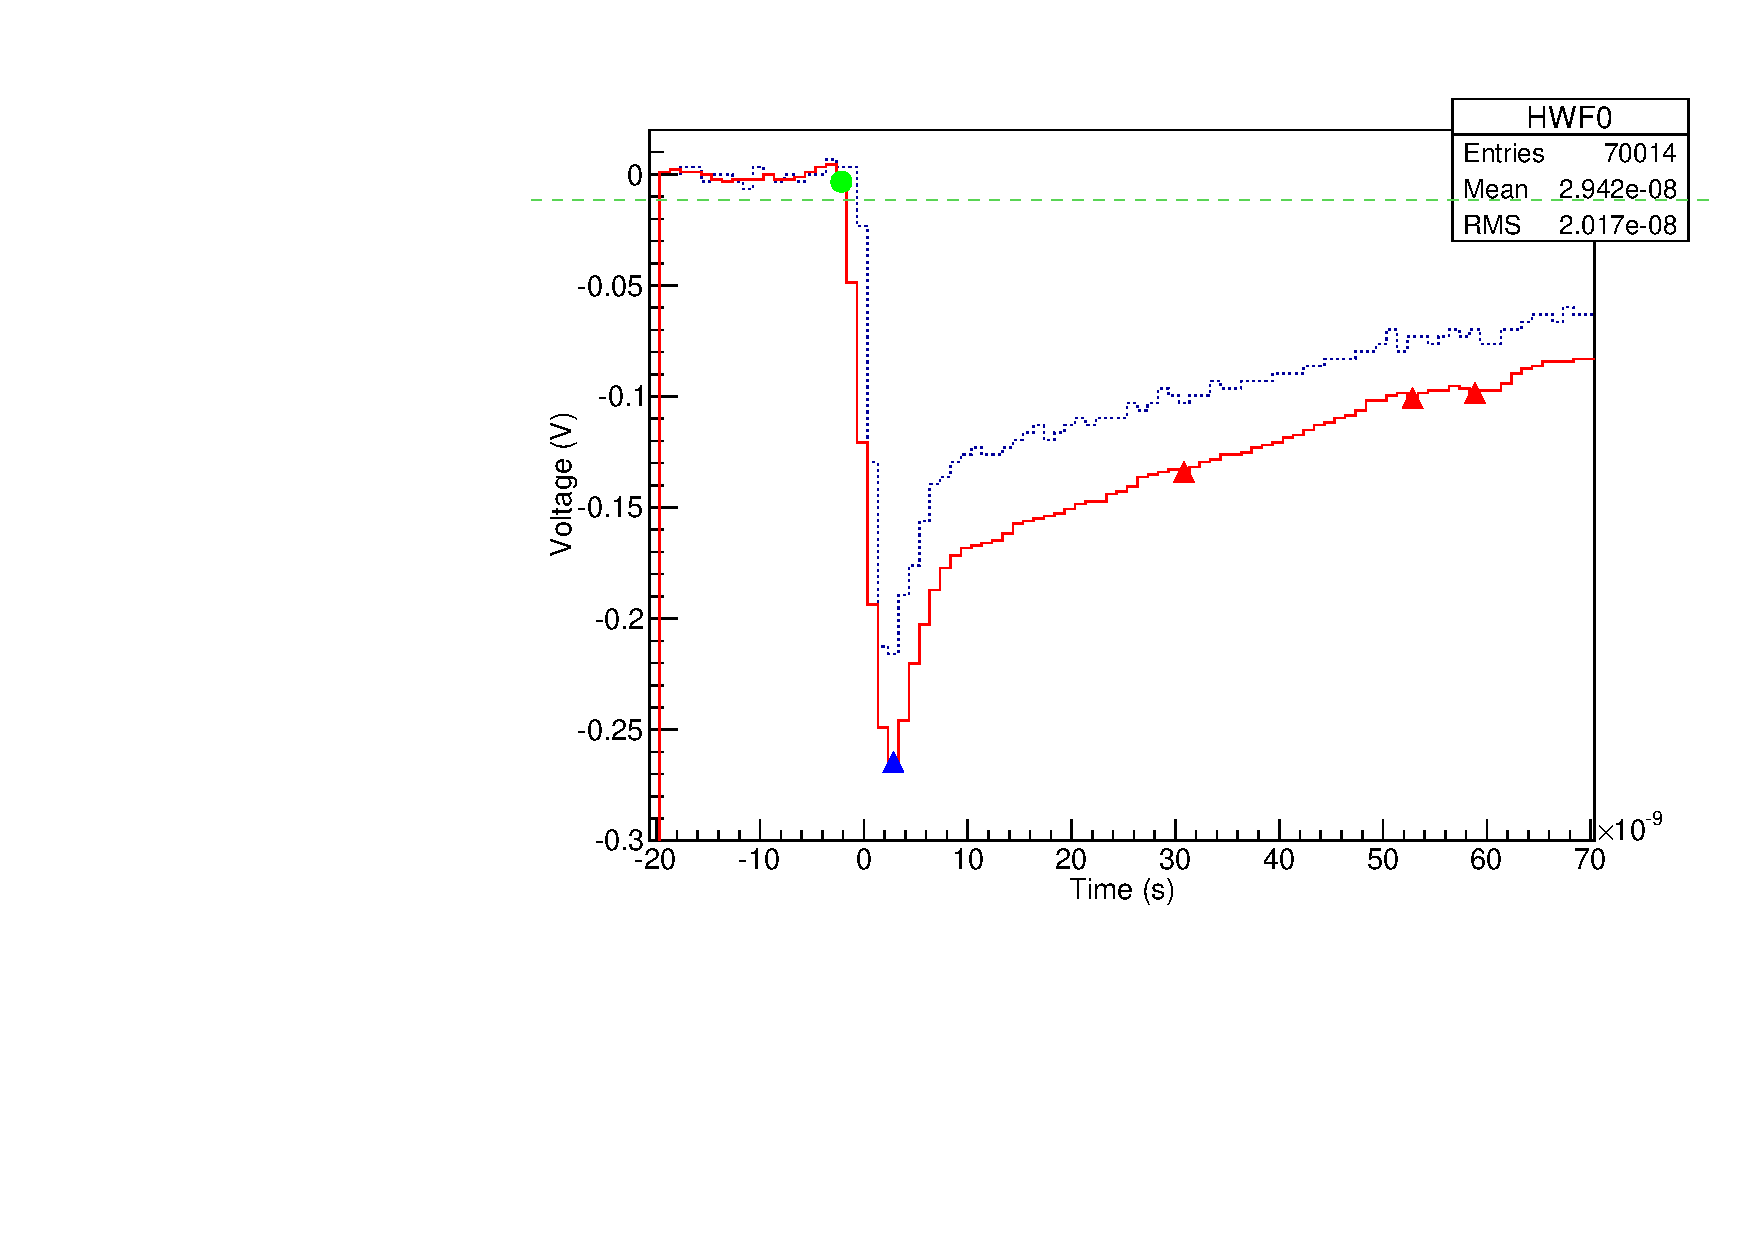
\includegraphics[height=0.38\textwidth]{peak_high.pdf}
\caption{At higher p.e., the amplitude bands are more spread out. These figures show this to be a result of inconsistent pulse shape.}
\end{figure}
\end{frame}

\begin{frame}{Delta Time}
\begin{figure}
\centering
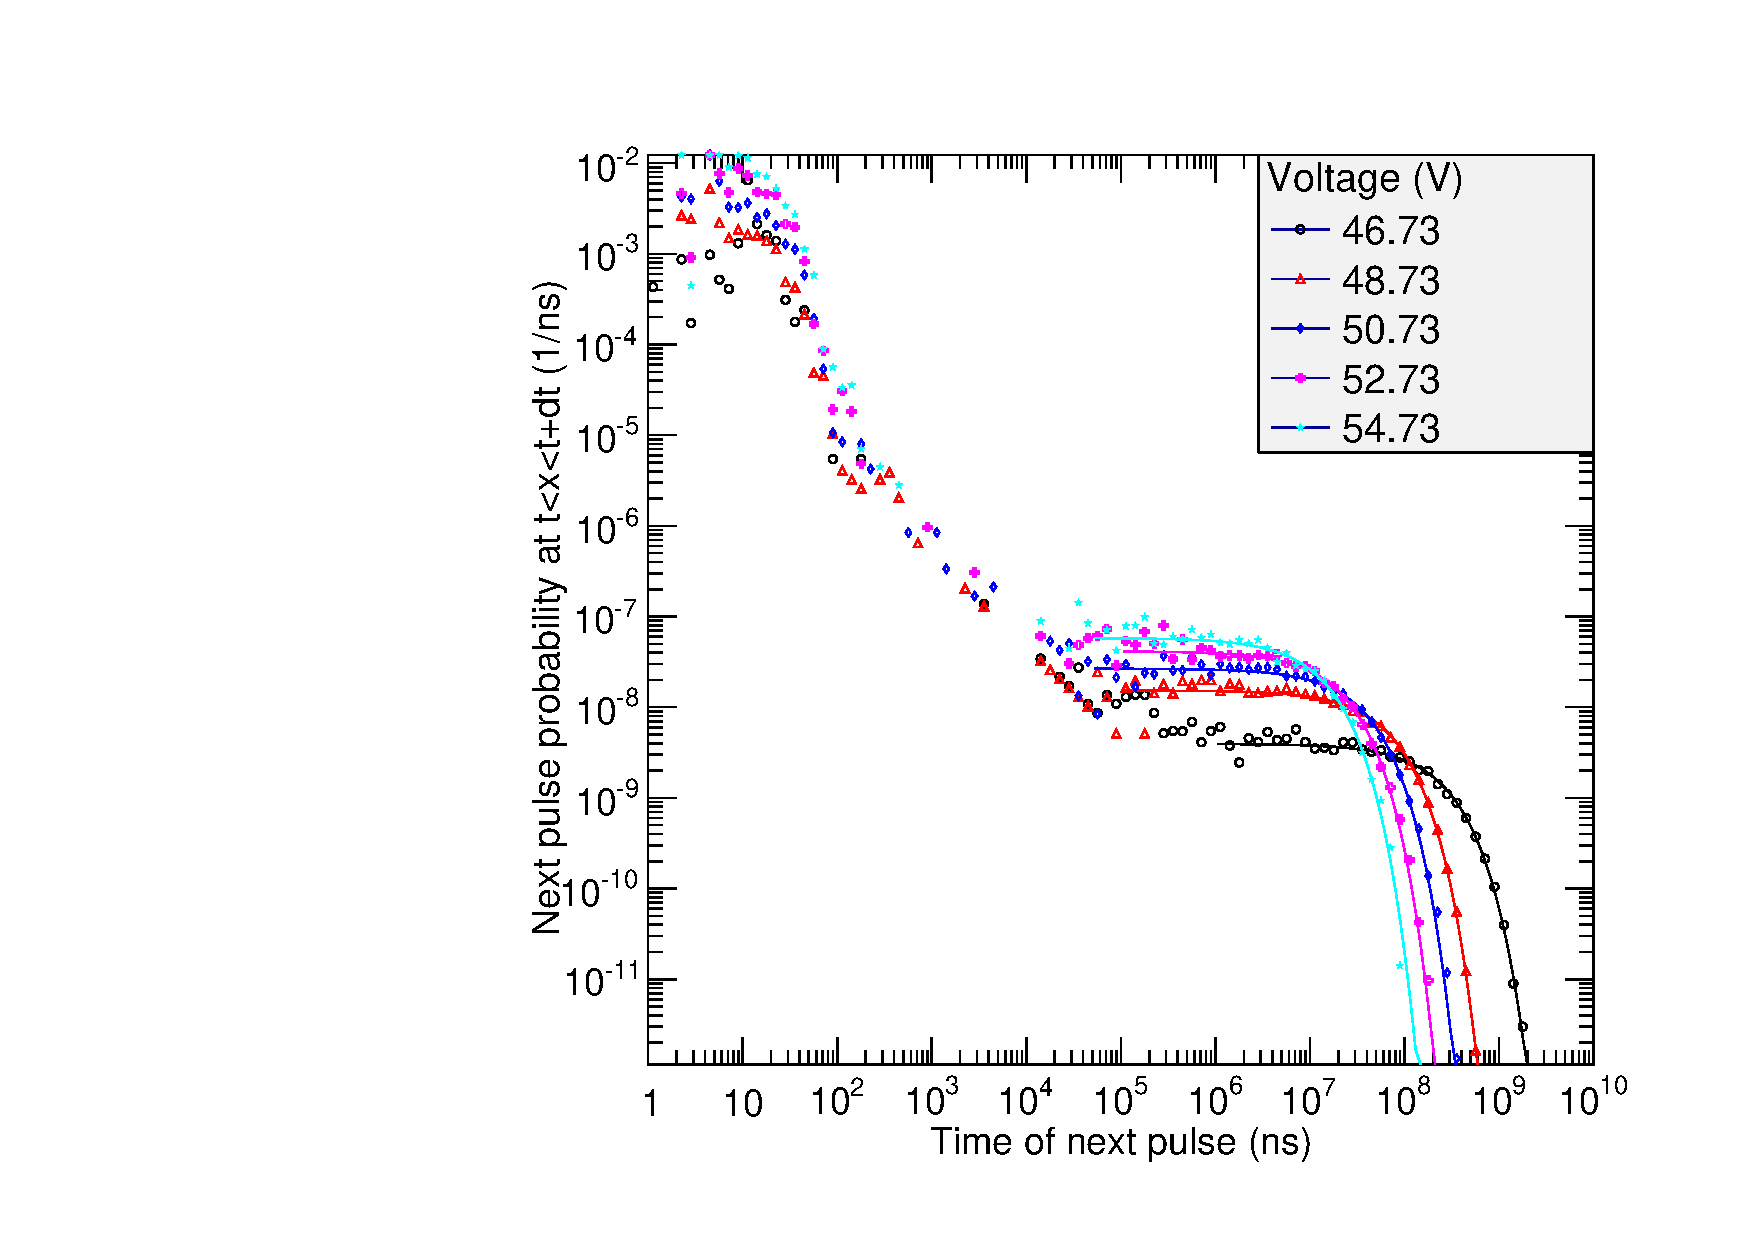
\includegraphics[height=0.5\textwidth]{deltatime.pdf}
\caption{Delta-time distribution for VUV3 at -100C at several operating voltages.}
\end{figure}
\end{frame}

\begin{frame}{Dark Noise Rate}
\begin{figure}
\centering
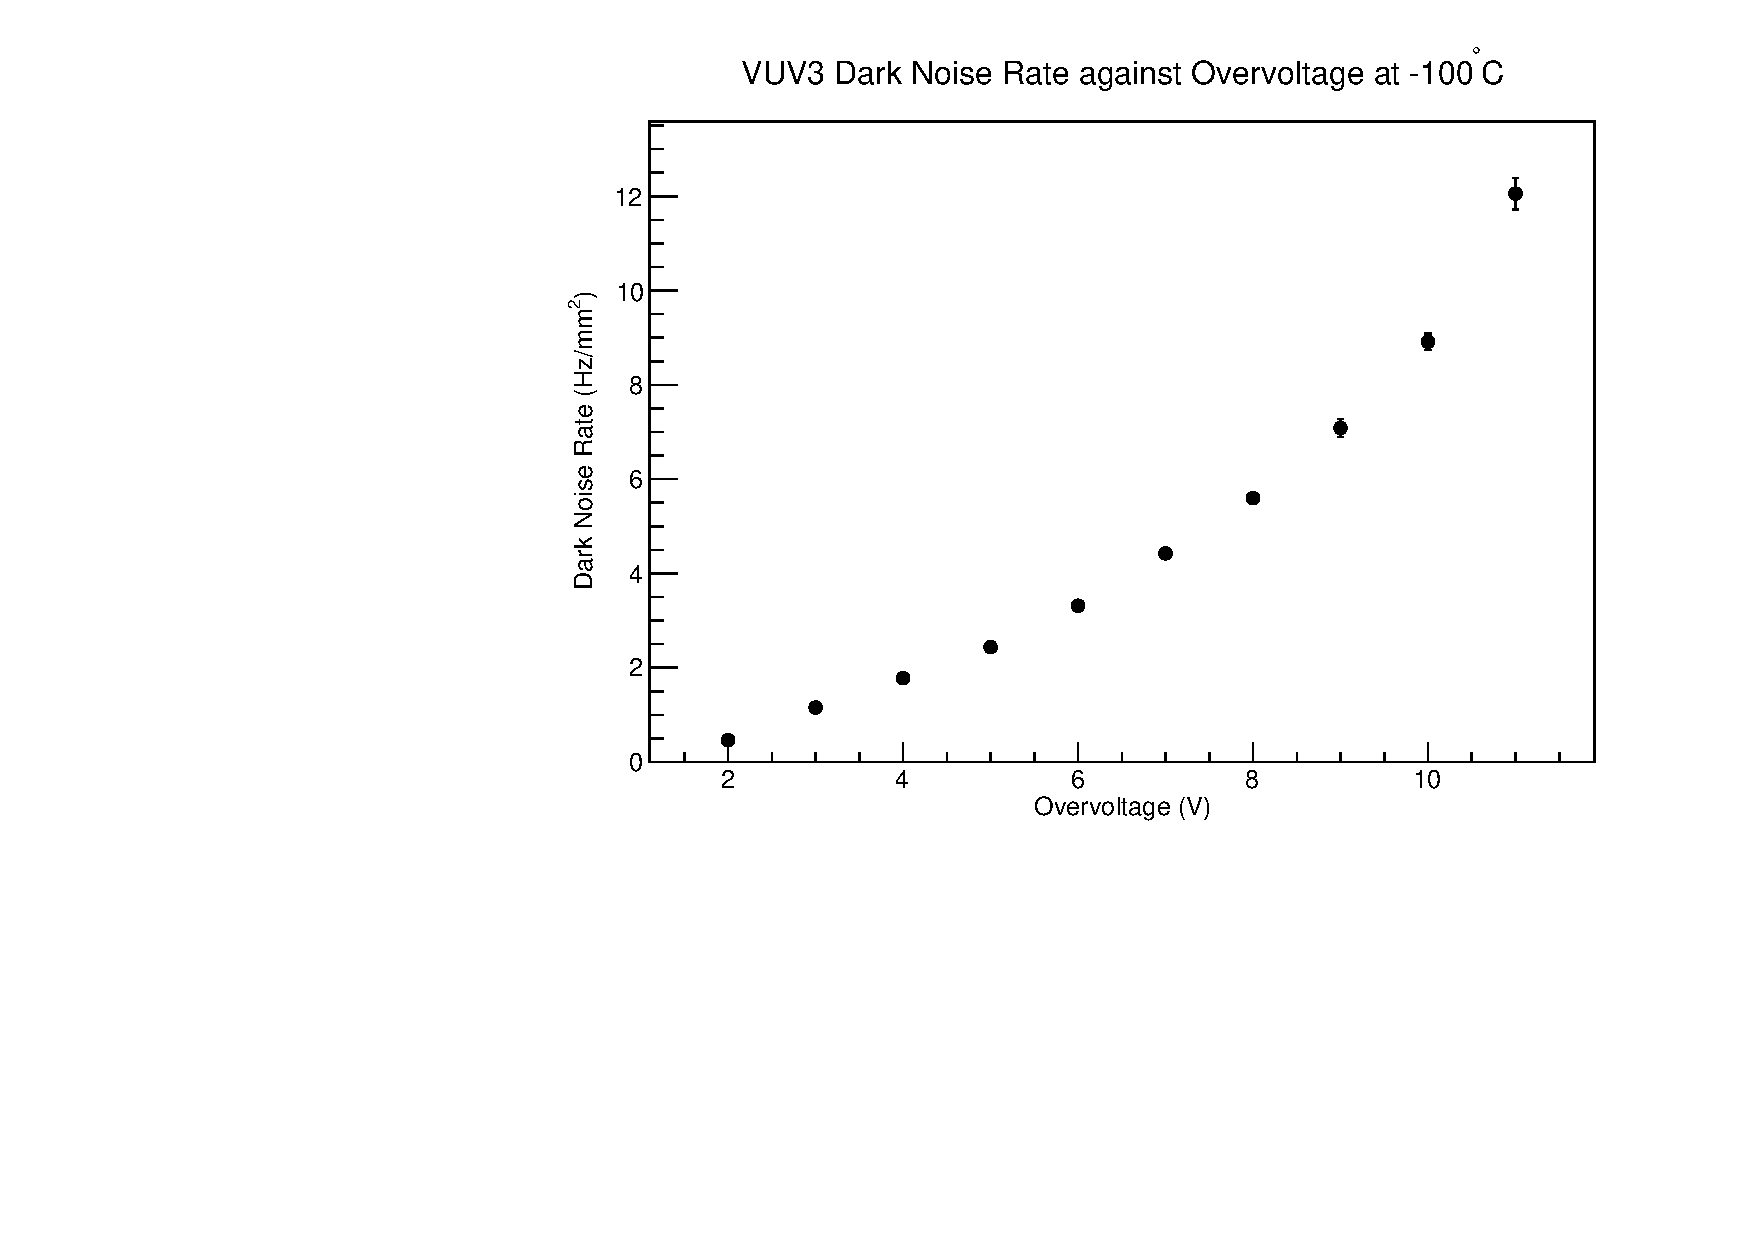
\includegraphics[height=0.5\textwidth]{VUV3_DN_vs_OV.pdf}
\caption{Dark noise rate against operating voltage for VUV3 at -100C. Extracted from fit to delta-time distribution.}
\end{figure}
\end{frame}

\begin{frame}{Afterpulsing Rate}
\begin{figure}
\centering
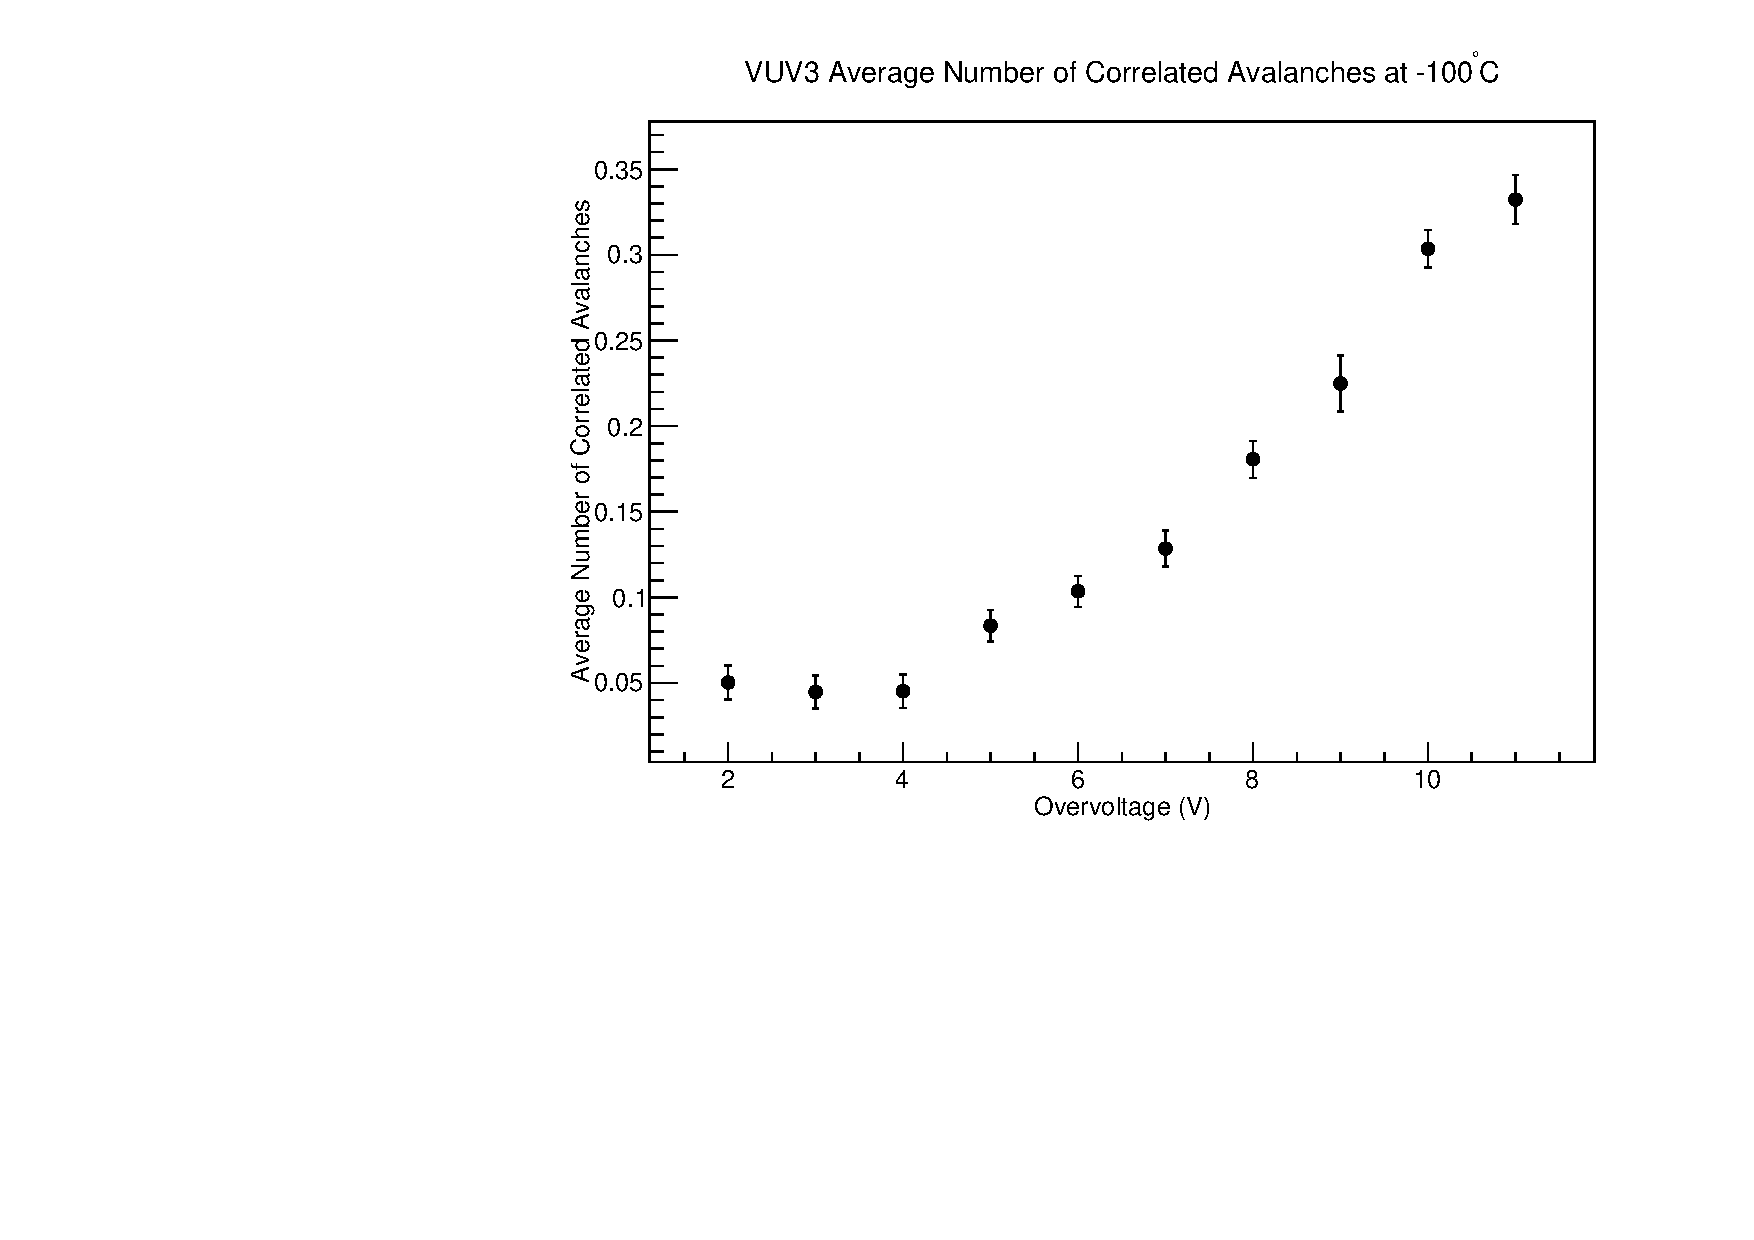
\includegraphics[height=0.5\textwidth]{VUV3_AP2_vs_OV.pdf}
\caption{Average number of afterpulses against operating voltage for VUV3 at -100C. Both values extracted from fit to delta-time distribution and counted directly.}
\end{figure}
\end{frame}

\begin{frame}{Crosstalk Rate}
\begin{figure}
\centering
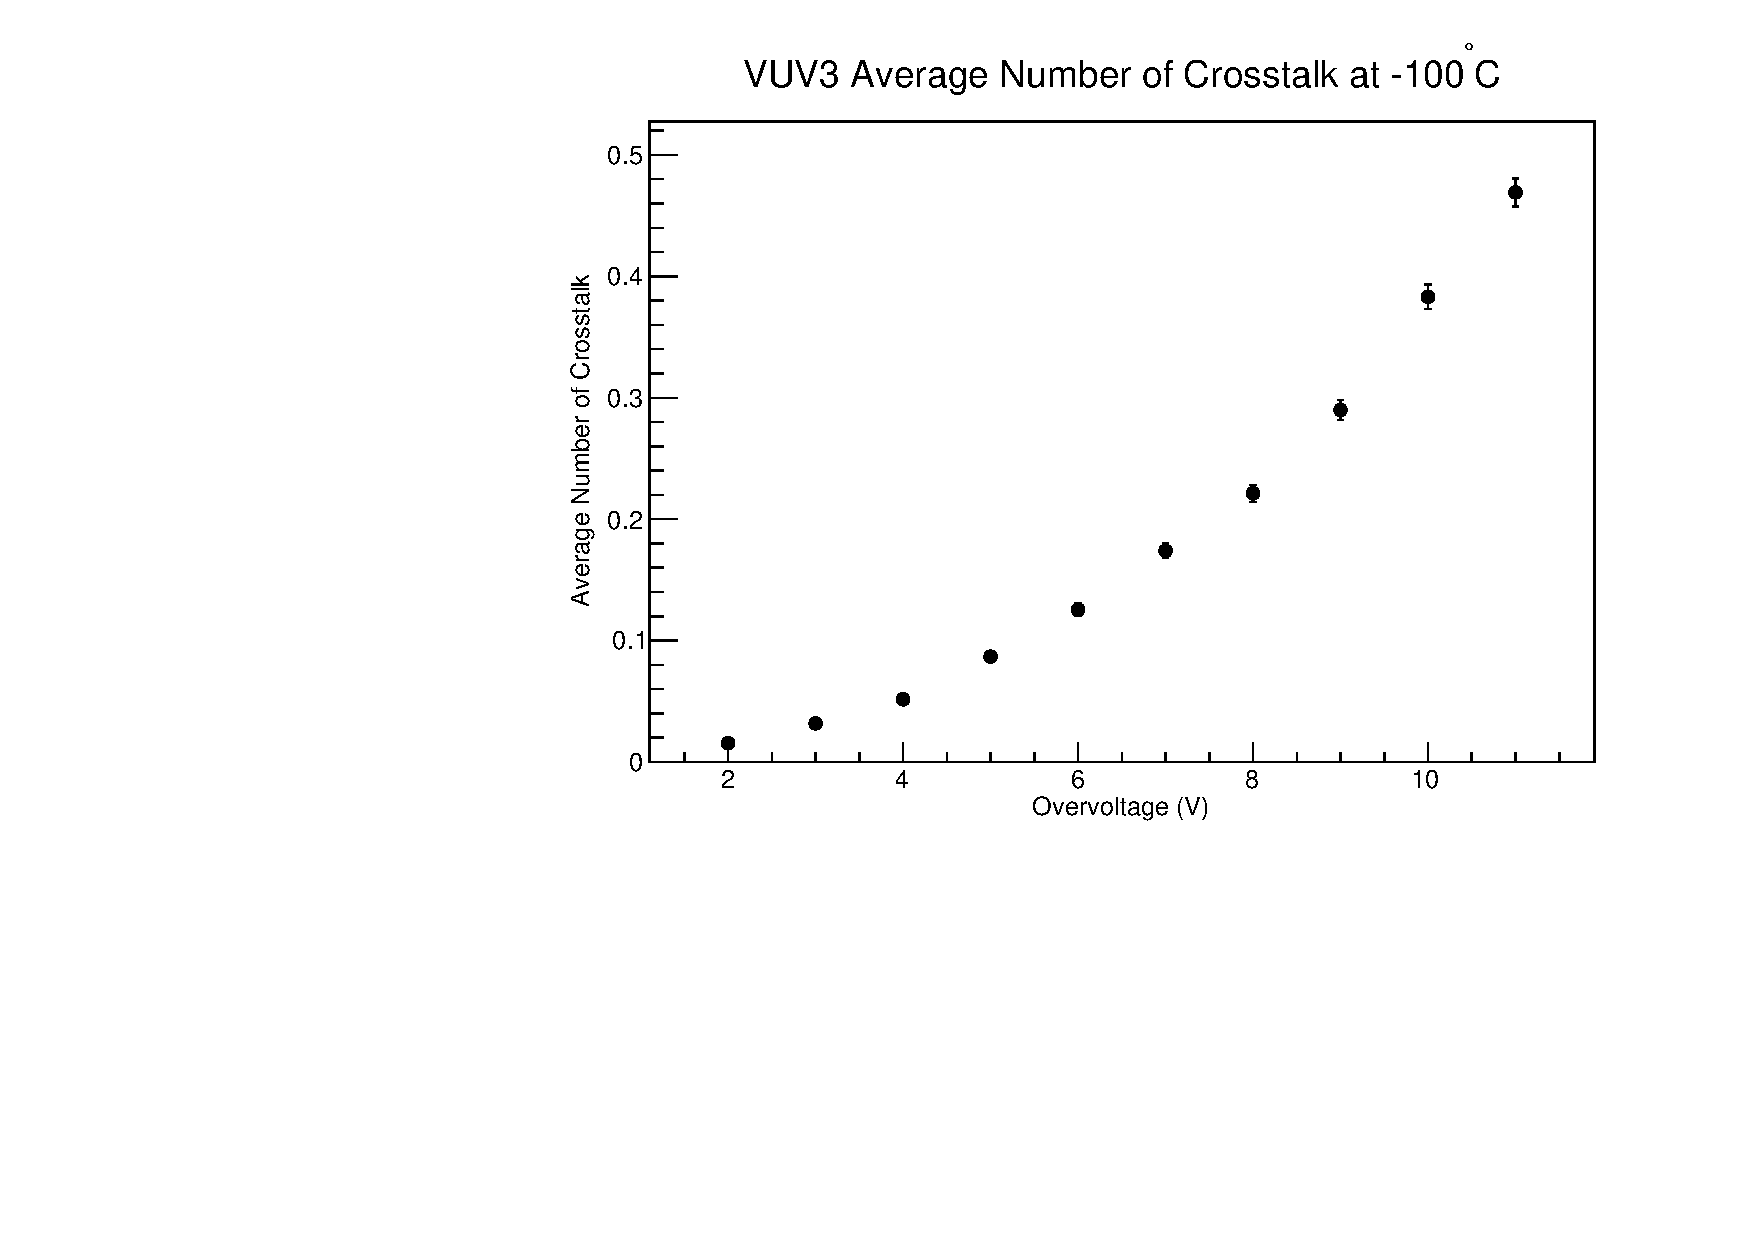
\includegraphics[height=0.5\textwidth]{VUV3_CT_vs_OV.pdf}
\caption{Average number of crosstalk against operating voltage for VUV3 at -100C. Calculated from counting process.}
\end{figure}
\end{frame}


\begin{frame}{Correlated Avalanches}
\begin{figure}
\centering
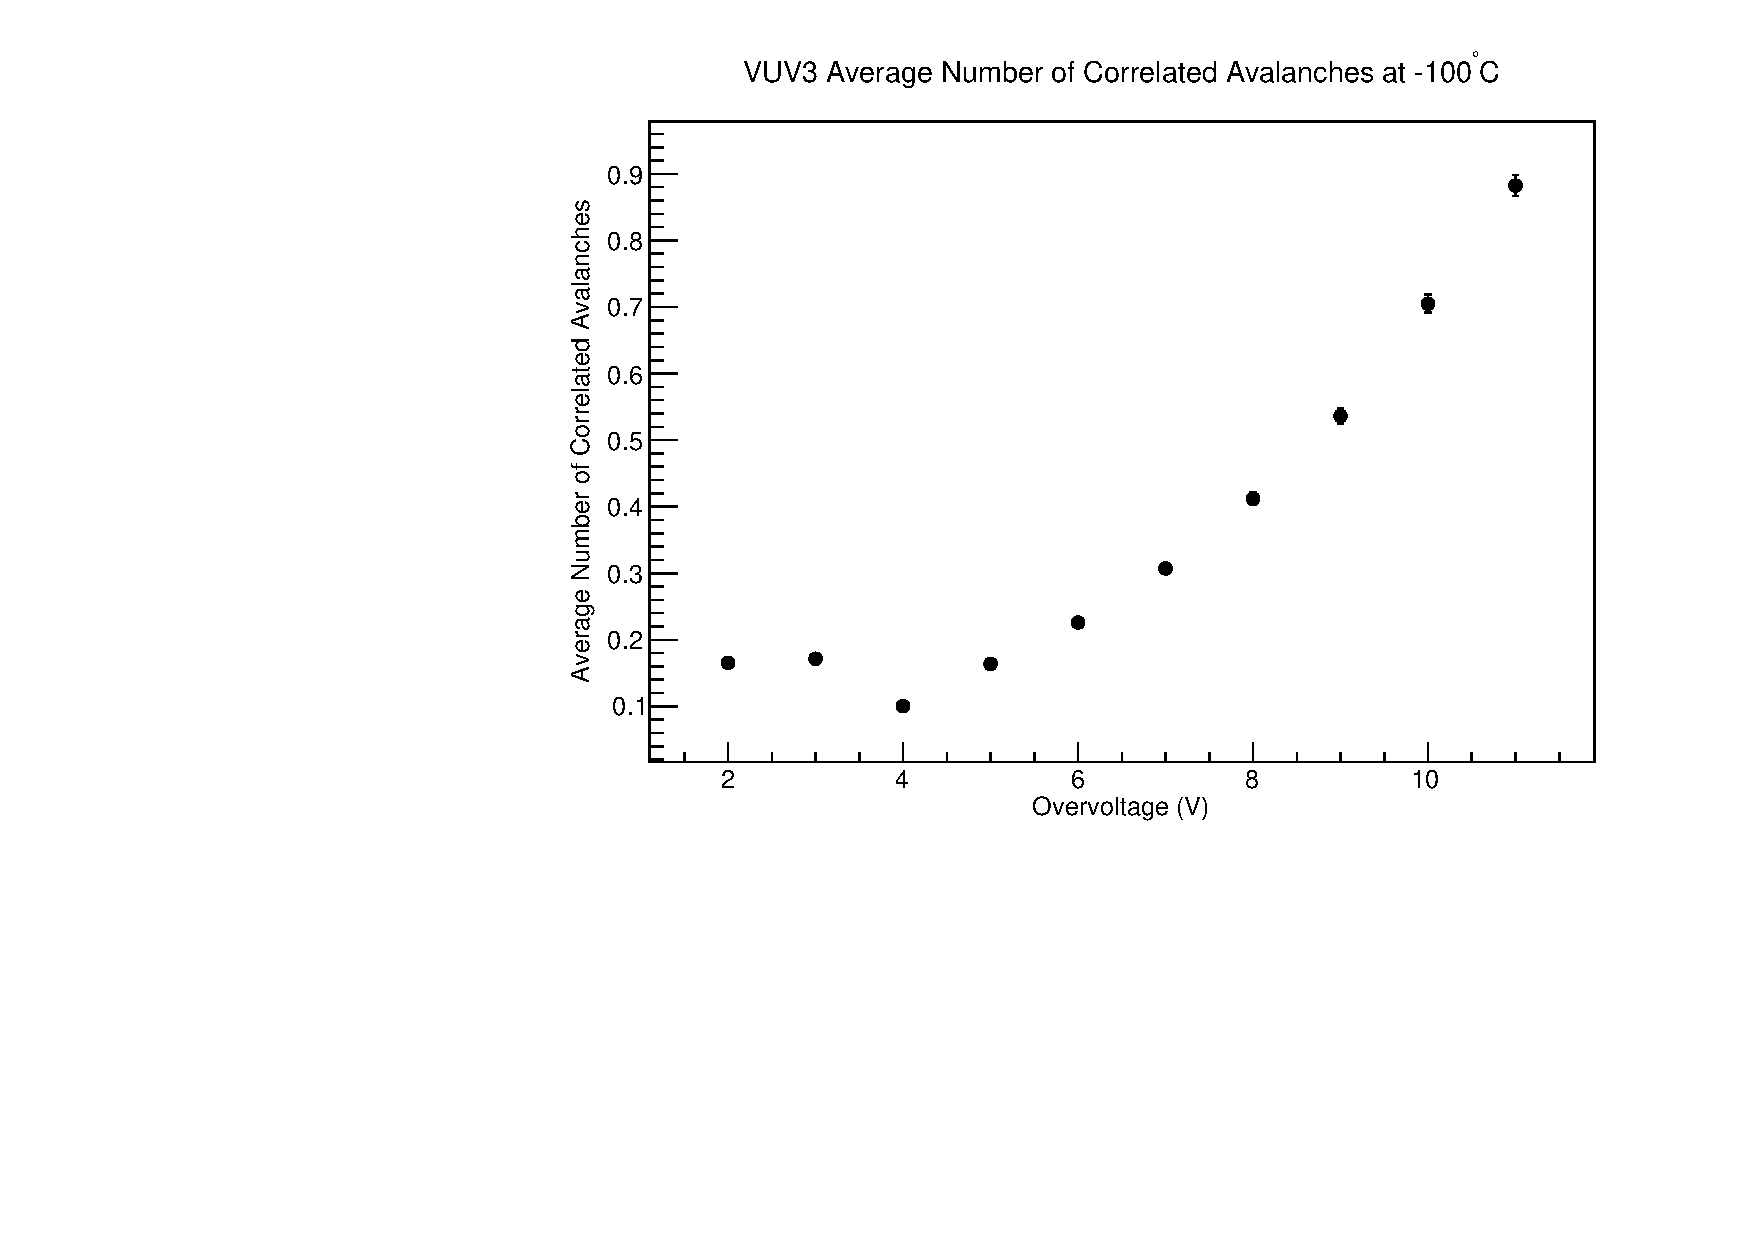
\includegraphics[height=0.5\textwidth]{VUV3_CA_vs_OV.pdf}
\caption{Average number of correlated avalanches against operating voltage for VUV3 at -100C. Sum of counted afterpulsing and crosstalk values}
\end{figure}
\end{frame}

\begin{frame}{<PE> Measurement}
\begin{itemize}
\item When the collimators were removed, the anticorrelation in <PE> was gone
\item To test if the UV filters had an impact, they were removed but the previous anticorrelation was still evident
\end{itemize}
\end{frame}

\begin{frame}{<PE> Measurement}
\begin{figure}
\centering
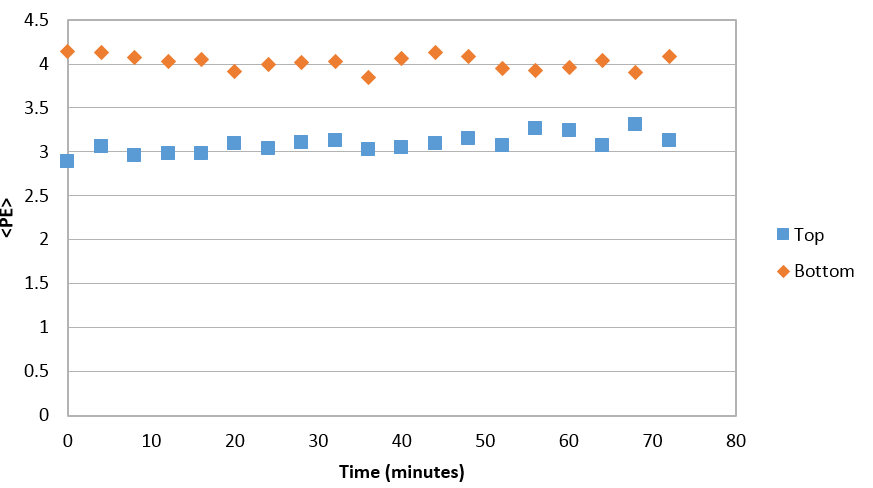
\includegraphics[height=0.5\textwidth]{PE.PNG}
\caption{PE measurement over time for VUV3}
\end{figure}
\end{frame}

\end{document}